\documentclass[utf8]{webofc}
\usepackage[varg]{txfonts}
% review
\usepackage[textwidth=120]{todonotes}
%\usepackage{color}
\usepackage{subcaption}

\begin{document}
    \title{Calculation of gain coefficient in Dwyer relativistic discharge feedback model of thunderstorm runway breakdown}
    \author{\firstname{Mikhail} \lastname{Zelenyi}\inst{1,2,3}\fnsep\thanks{\email{mihail.zelenyy@phystech.edu}} \and
        \firstname{Egor} \lastname{Stadnichuk}\inst{1,2}\fnsep\thanks{\email{egrstadnichuk@yandex.ru}} \and \firstname{Alexander} \lastname{Nozik}\inst{1,2}\fnsep\thanks{\email{altavir@gmail.com}}  
    }
    
    \institute{Institute for Nuclear Research of RAS
        \and
        Moscow Institute of Physics and Technology (State University) 
        \and
        Space Research Institute of RAS
    }
    \abstract{%
        Some of modern models used to describe TGF phenomenon and lightning ignition assume the existence of positive positron or gamma ray feedback. In this article we present some results of Monte-Carlo simulation of electromagnetic avalanches in atmospheric conditions and calculation of gain coefficient for both positron and gamma-ray feedback. The calculations were maid for realistic fields and acceleration cell sizes (up to 200 kV/m and 400 m respectively).
        The calculated gain coefficients for realistic fields and cell sizes are less than 10\% which strongly discourages use of positron and gamma feedback model to describe TGF phenomenon and other gamma-production mechanisms in atmosphere under normal conditions. The simulation also shows possibility of self-supporting positron feedback for extreme conditions like very high electric fields and very large cells.
    }
    %
    \maketitle
    
    \section{Introduction}
    Despite decades of investigations and observations, there are gaps in physics of atmospheric discharge. Nowadays the process of development of lightning after initial breakdown is widely known. However, the mechanism of cloud ionization which is required to produce initial breakdown is not described accurately. Furthermore, some observed effects connected to lightning generation also lack explanation. For example, terrestrial gamma ray flashes (TGFs) are closely correlated with thunderstorms. This phenomenon has several models but none of them are considered satisfying.
    \begin{figure}[ht!]
        \begin{subfigure}[b]{0.5\textwidth}
            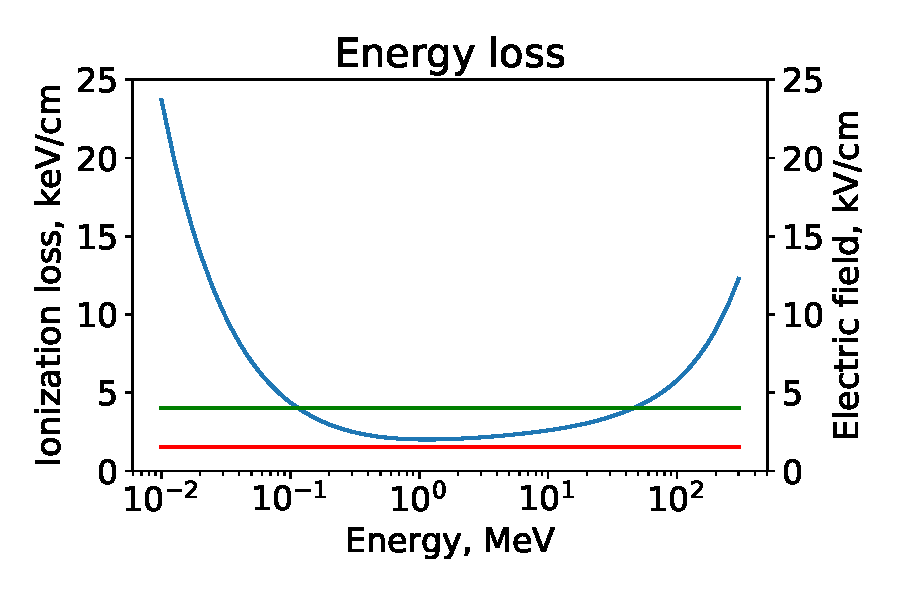
\includegraphics[width=0.95\linewidth]{pictures/01_Gurevich}
            \caption{}
            \label{pic-gurevich-a}
        \end{subfigure}
        ~
        \begin{subfigure}[b]{0.5\textwidth}
            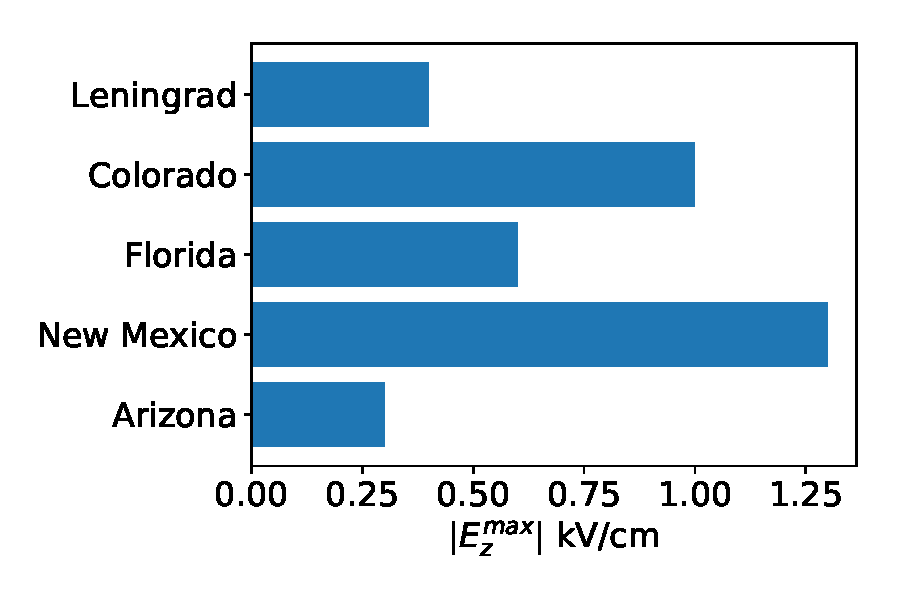
\includegraphics[width=0.95\textwidth]{pictures/03_extremal_field}
            \caption{}
            \label{pic-field-b}
        \end{subfigure}
        \caption{
            a) Gurevich model: if electric field is higher than MIP loss (green line) there are possible to generate runway electron, otherwise (red line) avalanches are  discharged~\cite{gurevich1992runaway}.
            %     a) Distribution of horizontal electric field ~\cite{mazin1989clouds} 
            b) Extremal value of vertical electric field (before 1989 y.)~\cite{mazin1989clouds}}
    \end{figure}
    
    Gurevich has made a notable contribution in understanding of electron avalanche physics in atmosphere~\cite{gurevich1992runaway}. According to his research, cosmic ray charged particles are accelerated in thundercloud electric field and produce enhanced ionization. Gurevich studied electron behavior in air with electric field. Energetic electrons that are able to accelerate under such conditions are called runaway electrons (see Fig.~\ref{pic-gurevich-a}). In the following works, Gurevich developed the runaway theory~\cite{gurevich1999lightning,gurevich2001kinetic}. Nevertheless, the flux of cosmic rays is not intensive enough to explain cloud charging with only runaway electron ionization.
    \begin{figure}[t]
        \centering
        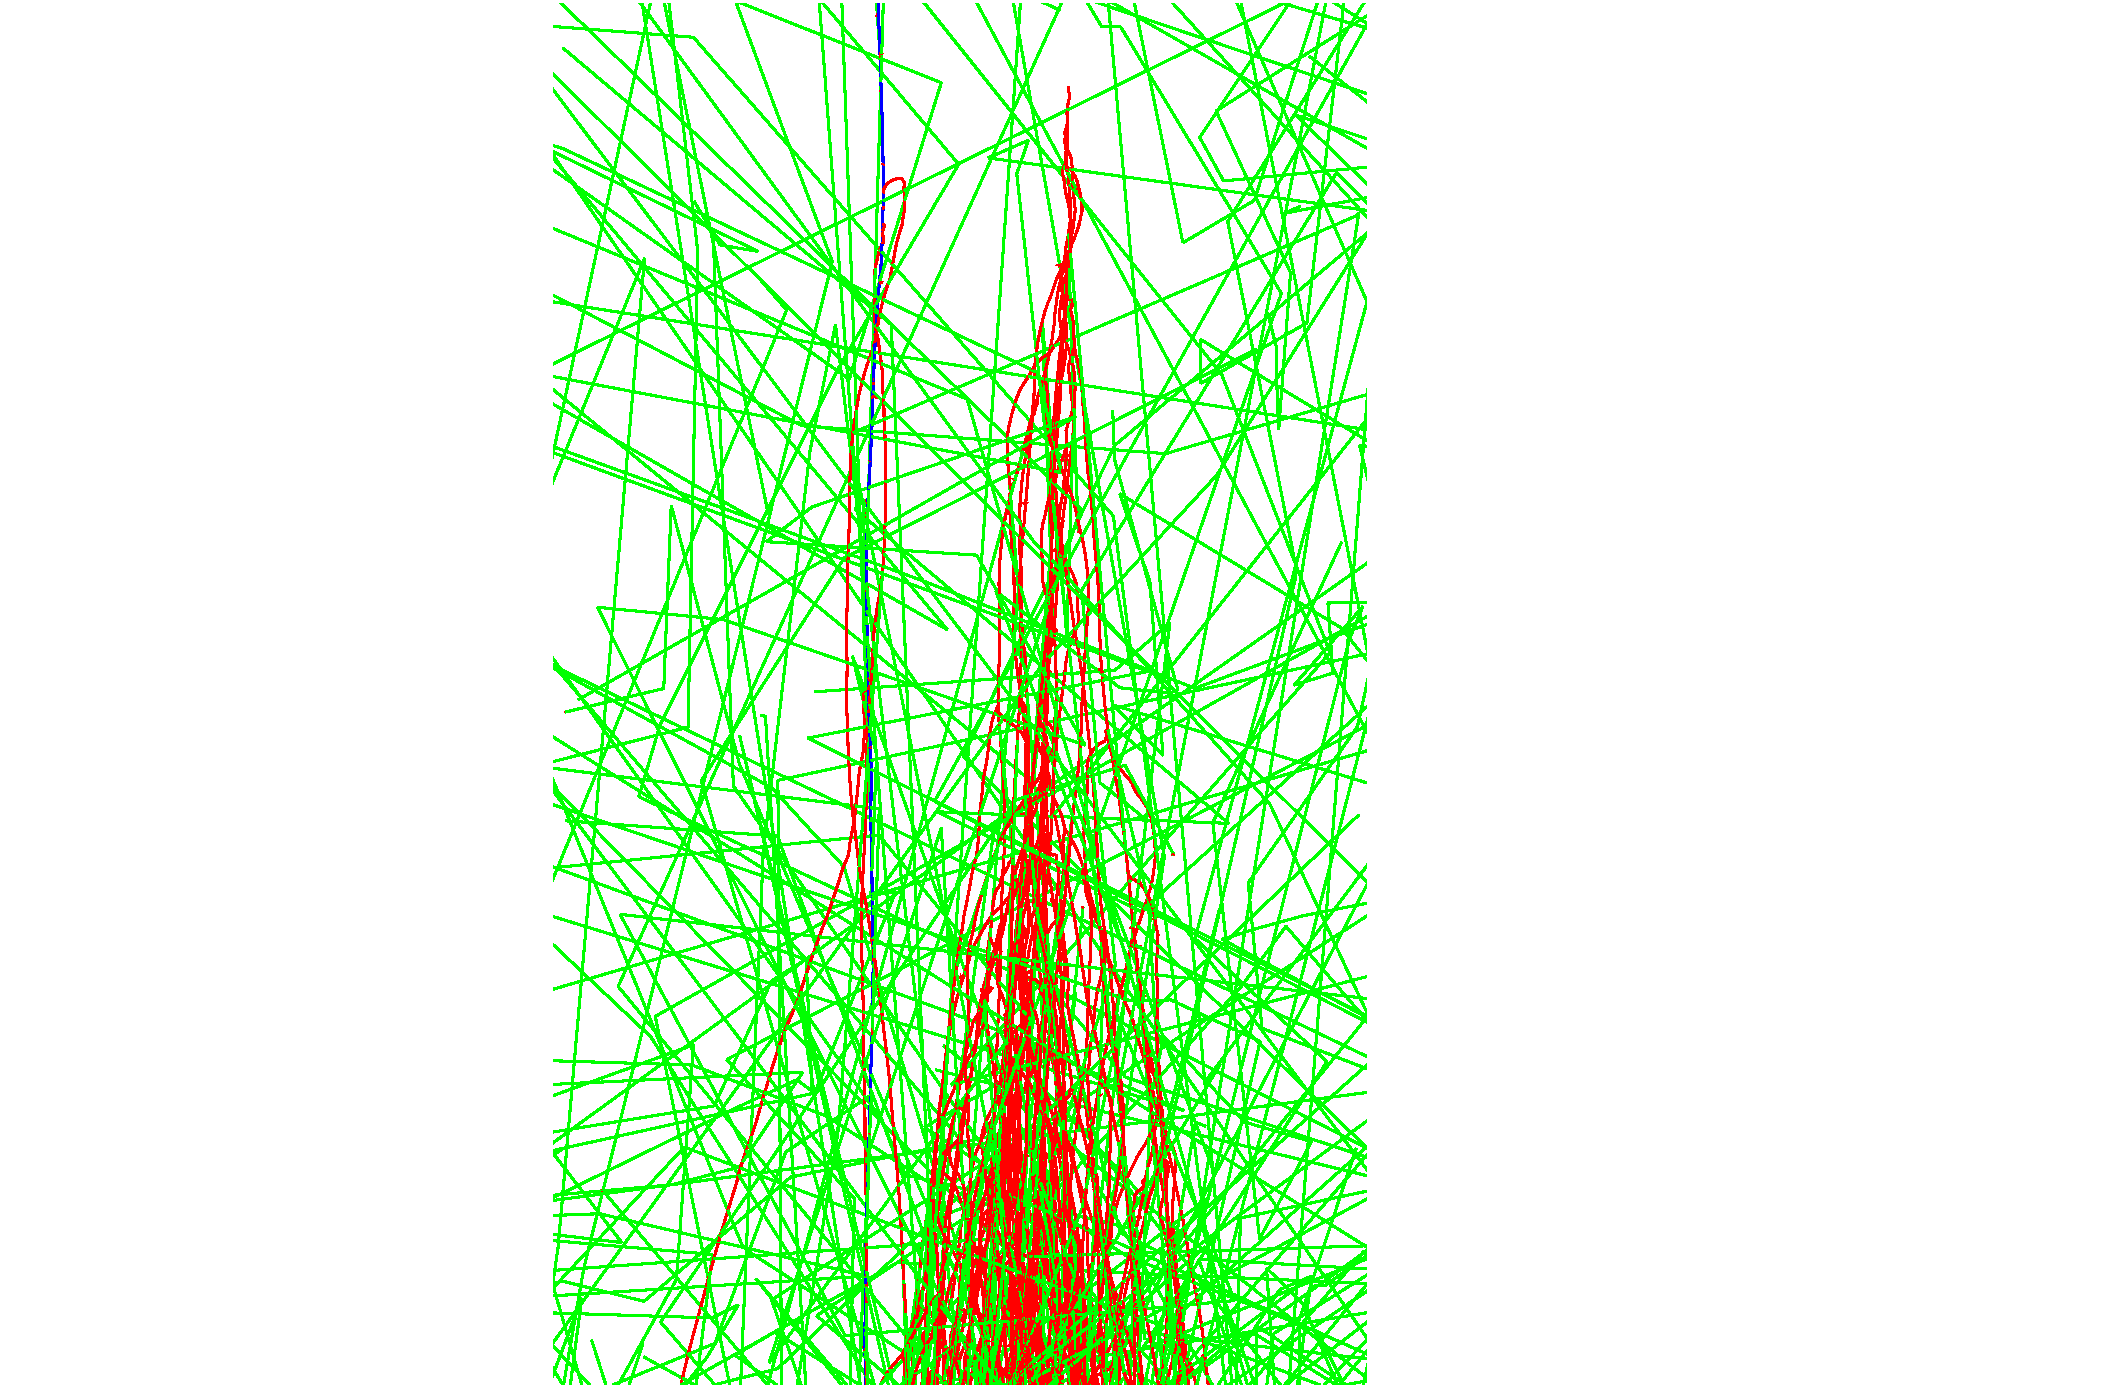
\includegraphics[width=0.5\textwidth]{pictures/10_dwyer}
        
        
        
        \caption{Geant 4 simulation. Red tracks~--- electrons. Blue tracks~--- positrons. Green tracks~--- gamma-rays. Simulation conducted for normal air density and electric field of $10~kV/cm$. Left blue track is a positron which generates new runway avalanche and illustrates positron feedback mechanism.}
        \label{pic-dwyer-a}   
    \end{figure}
    
    Dwyer proposed a mechanism of positron feedback that increases the runaway electron flux~\cite{dwyer2003fundamental}. Dwyer constructed his simulation in the cell with electric field value of 1000 kilovolts per meter. The cell is a cylinder of air with electric field. Dwyer’s feedback mechanism is described briefly as follows. A runaway electron propagating through such a cell radiates bremsstrahlung photons. If the bremsstrahlung photon has enough energy, then it can produce an electron-positron pair. The positron charge is opposite to the electron one, therefore it reverses in electric field and then propagates in direction opposite to the direction of runaway electron motion. Such positrons have a chance to produce electrons near the beginning of primary runaway electron track. Then ionization electrons can reverse in the electric field and propagate through cell creating secondary electron avalanche. The runaway theory with Dwyer feedback mechanism is considered to be one of the most reliable theories describing processes appearing in thunderclouds before lightning strike. An example of Dwyer mechanism is shown at Fig.~\ref{pic-dwyer-a}.
    
    Direct measurements show that observed thundercloud electric field is less than 200 kilovolts per  meter~\cite{mazin1989clouds, marshall1995electric}. Some data points are showed at Fig.~\ref{pic-field-b}. However, there are no results in the literature regarding how positron feedback works under such conditions. The aim of the present work is to reveal whether Dwyer model operates in cells with uniform electric field less than 200 kilovolts per meter and air density between 0.3 and 0.8 kilogram per cubic meter and to calculate positron feedback coefficients for different electric fields. %The algorithm of feedback coefficient calculating is described in methodology section.
    %The results of the investigation are negative. The paper shows that positron feedback coefficient is much less than 1 in cells with electric field under 200 kilovolts per meter. That means that one electron avalanche does not create secondary avalanches by positron feedback mechanism. The accurate value of positron feedback coefficient is stated in results section.
    \section{Simulation}
    \label{sec:Sim}
    In this work we consider two mechanisms proposed by Dwyer: gamma and positron feedbacks. 
    In both cases the idea is similar:
    \begin{enumerate}
        
        \item Initial electron accelerates in the electric field and produces photon which is flying backwards or positron which is reversed by the electric field and also is flying backward.
        
        \item The positron or photon produces an electron near the beginning of the acceleration cell.
        
        \item This electron is rotated by the electric field and produces the secondary avalanche. 
        
    \end{enumerate}
    
    The electron produced in the last phase is called secondary electron. The gain coefficient is defined as an average number of secondary electrons produced per single initial electrons. Obviously, in order to have significant enhancement mechanism, one need gain to be greater or equal to 1. 
    The gain is obviously proportional to the number of positrons and/or gamma rays generated by the initial electron, but there is a number of factors that contribute to that quantity.
    
    \begin{itemize}
        \item Positrons are mostly produced not directly, but by bremsstrahlung gamma rays emitted by initial electron. The mean free path of this gamma for this process is quite large (of the order of few kilometers for atmospheric conditions). Therefore, the probability of generating positron inside the acceleration cell is proportional to cell size and density (increase in density reduces the mean free path). Also, the number of positrons is proportional to the field in the cell (since electrons with higher energy are more likely to produce appropriate photons).
        \item Not all positrons are accelerated backwards. Due to conservation of momentum, large fraction of them are moving forward. Those positrons are usually stopped by the electric field and annihilated.
        \item Accelerated positron has rather small probability to directly produce an electron because the cross-section diminishes with energy.
        \item Secondary electrons, produced both by positrons and gamma rays usually fly toward "back" side of the cell due to conservation of momentum. Those electron could be rotated by the electric field to fly forward, but one must remember, that once electron energy is below Gurevitch's critical energy, it could not be accelerated and is lost.
    \end{itemize}
    
    The simulation are done by GEANT4 transport code \cite{ALLISON2016186} in three steps:
    
    \begin{enumerate}
        \item Calculate energy and angular spectra of positrons and gamma rays of sufficient energy, which are produced inside the cell.
        \item Use those spectra as initial distributions for secondary simulation of particles flying backwards and register all secondary electrons.
        \item Select only those electrons, which could be later reversed forward without stopping. Minimal particle energy is determined from the value of electric field and ionization loss curve (\ref{pic-gurevich-a}). The dependence of minimal angle between cell axis backward direction and velocity is shown at Fig.~\ref{pic-reverse-b}.  All of electrons situated above the curve are able to generate secondary electron avalanche in the cell. According to this graph, less than 50\% of electrons produced by positrons will generate secondary electron flux.
    \end{enumerate}
    \textit{G4EmStandard} physics list was used for simulation This physics list provides a compromise between accuracy and speed of simulation (for comparison physics list \textit{G4EmStandard\_opt4} has better algorithm of particle tracking, but requests more time and gives similar results for simulation parameters which were considered in this work). Also energy of particles is rather so it is possible not to use low-energy physics list as \textit{G4EmPenelopePhysics} and \textit{G4EmLivermorePhysics}. Low energy cut off is 0.5 MeV in the simulation.
    
    
    
    \section{Results}
    
    \begin{figure}[ht!]
        \begin{subfigure}[b]{0.5\textwidth}
            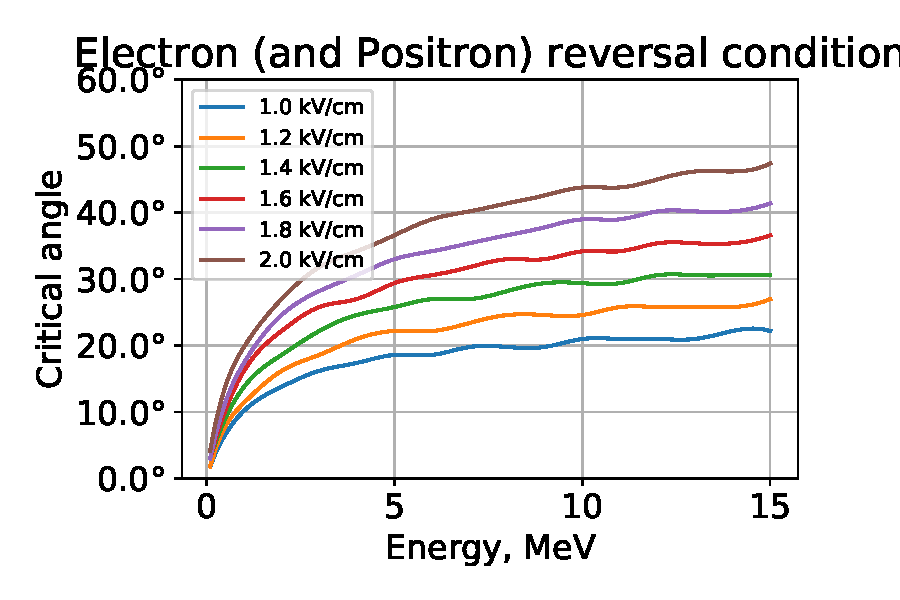
\includegraphics[width=0.95\linewidth]{pictures/09_condition}
            \caption{}
            \label{pic-reverse-b}
        \end{subfigure}
        ~
        \begin{subfigure}[b]{0.5\textwidth}
            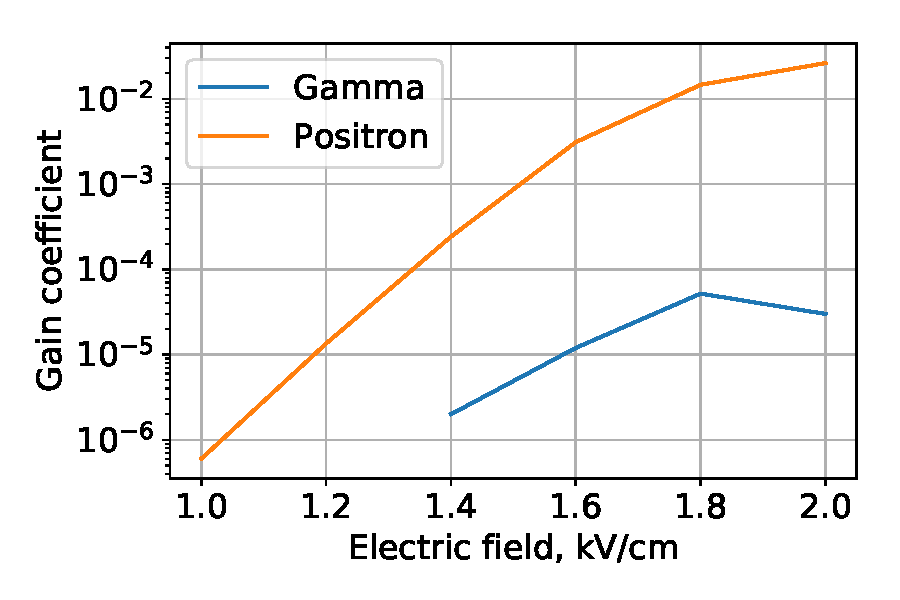
\includegraphics[width=0.95\textwidth]{pictures/08_gain}
            
            \caption{}
            \label{pic-gain-a}
        \end{subfigure}
        \caption{ a) Minimum reversal angle between electron motion direction in moment of its birth and electric field depending on electron energy.
            b) Positron (gamma) feedback coefficient in dependence on cell electric field for next parameters: primary electron energy~--- $3~MeV$, field area size~--- $400~meter$, electric field from $1$ to $2~kV/cm$, air density~--- $0.5~kg/m^3$ ($\sim 0.5~atm$).
        }
    \end{figure}
    
    The gain coefficient is calculated as a convolution of probabilities of producing valid particle on each step and applying all relevant cuts.
    
    Using simulation result we calculate gain coefficient by description from section ~\ref{sec:Sim}. The result for the following cell parameters: primary electron energy~--- $3~MeV$, field area size~--- $400~meter$, electric field from $1$ to $2~kV/cm$, air density~--- $0.5~kg/m^3$ ($\sim 0.5~atm$) is presented at Fig.~\ref{pic-gain-a}. It can be clearly seen that the total gain factor is significantly smaller than one for fields less than $200~kV/m$. The gamma gain and positron gain are slight and don't exceed 10\%. Such small number could not explain self-sustaining discharge mechanism, proposed by Dwyer and gives only small contribution to the total charge generation.
    
    One should note, that Dwyer mechanism could still work for higher fields (like $1000~kV/m$), but those conditions are unreachable, because normal gas breakdown in moist (and even dry) air starts much sooner. Experimental evidence shows that it is not the case in thunderclouds.
    
    The model shows a positron annihilation line in gamma-spectrum, which was observed in multiple experiments~\cite{dwyer2015positron}. This line is an intrinsic part of any model based on Gurevitch runaway model, still this positron line does not guarantee the role of positrons in producing the feedback. Detailed numerical estimation of those effects requires additional simulation with enhanced statistics which will be performed in the near future.
    
    \section{Conclusion}
    
    The results of GEANT4 simulations, presented in this article clearly show that positron and gamma feedback introduces very small (few percents at most) contribution to total charge generation in the thundercloud under realistic conditions (electric field between $100$ and $250~kV/m$ and pressure from $0.5$ to $0.8~atm$). 
    
    Dwyer positron enhancement is still possible for much higher electric fields (like $1000~kV/m$), but those fields are unreachable in the thunderclouds since they are higher than the breakdown field. The simultaneous increase of field and density proposed in one of the works by Dwyer~\cite{dwyer2003fundamental} conserves Gurevitch's critical energy but strongly affects the number of produced positrons (both changes work in direction of increasing positron flux).
    
    This work is supported by the Russian Science Foundation under grant No. 17-12-01439.
    
    \bibliography{references}{}
\end{document}
